\section{The Plug-In}
Introduction to the chapter.
Something about we first explore the user interface of the plugin, and then we look into the elements consisting within the user interface.

	What elements are there in this chapter?	
		User Interface
			All teh stuff the user can do in this plugin with pictures.	
		EasyInsert
			plug-in specific elements for RWS and how they are used.
			.ui was not used, why?
		Dialogs
		EasyInsert Construction - Bringing it all together.	
		Settings			
		Device tab
			mention something in the introduction about how the tabs will be gone through
		Geo tab
		Delete tab
		

\subsection{User Interface}
\label{sec:UserInterface}
This section explores the user interface of the plugin. When the plugin is loaded and opened, the user is met with figure~\ref{fig:EasyInsertDevice}. This is the Device tab of EasyInsert and from here it is possible to select a device listed and load it into the WorkCell by pressing the Load button. Upon pressing Load, the user is prompted with a dialog window where the user can specify options about the loaded device. Figure~\ref{fig:loadDialog} is the exact dialog window the user would see after selecting a device and pressing the load button. The user can now give the device a unique name, select a frame that the device should be on and specify the configurations such as displacement and rotation. A user can now select e.g. a fanuc robot arm, as the one on figure~\ref{fig:FANUCLRM200}, and insert it. Afterwards the user can then select another device, let's say some kind of hand device, and now insert that device on the end frame of the fanuc. The hand device now acts as the end effector of the fanuc, which only took a few clicks to set up. 

\begin{figure}[h] % 3 figures of the tabs
        \begin{subfigure}[b]{0.32\textwidth}
                \centering
                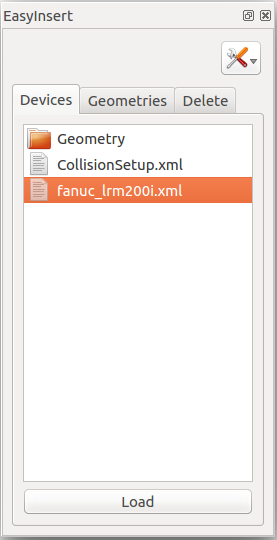
\includegraphics[width=.95\linewidth]{Figures/EasyInsertDevice.png}
  				\caption{Devices}
 				\label{fig:EasyInsertDevice}
        \end{subfigure}%
        \begin{subfigure}[b]{0.32\textwidth}
                \centering
                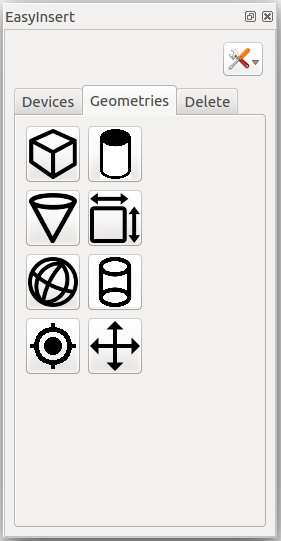
\includegraphics[width=.95\linewidth]{Figures/EasyInsertGeo.png}
  				\caption{Geometries}
  				\label{fig:EasyInsertGeo}
        \end{subfigure}%
        \begin{subfigure}[b]{0.32\textwidth}
                \centering
                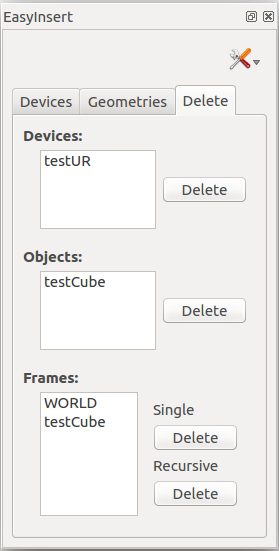
\includegraphics[width=.95\linewidth]{Figures/EasyInsertDelete.png}
  				\caption{Delete}
  				\label{fig:EasyInsertDelete}
        \end{subfigure}%
        \caption{The three tabs a user can interact with in the plugin. In Devices it is possible to select and load a device. In Geometries the user can click an icon (representing a geometry) which then prompts a dialog window with options regarding the insertion of said geometry. In Delete a user can select either a Device, Object or Frame to delete it.}\label{fig:EasyInsertTabs}
\end{figure}

It should be noted, that the first time EasyInsert is loaded and opened, the device tab shows the root content of the operating system. Thus the user needs to change the path of the list shown in the Device tab to a path containing any desired devices. In the right top corner of the plugin is a tool bar button (the only button in the tool bar so far) called settings. Clicking this button and choosing Libraries will prompt the user with the dialog window on Figure~\ref{fig:settingsDialog}. The user can here see what path is used and change it with the [...] button. The [...] button shows a new dialog window where the user can navigate his/her OS and specify the path that should be shown in the device tab.\\

\begin{figure}[h] % 3 figures of dialog windows
     \centering
     \begin{subfigure}[b]{0.45\textwidth}
	  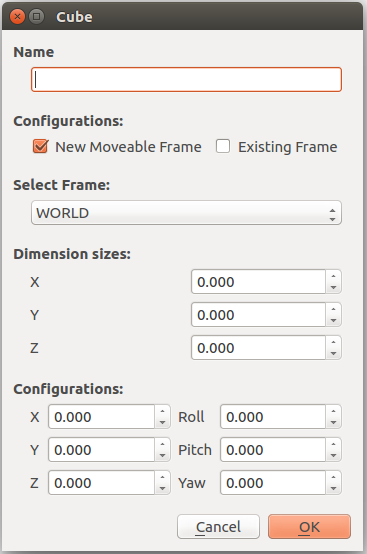
\includegraphics[scale=0.7]{Figures/EasyInsertCubeDialog.png}
       \caption{Cube insertion dialog window}\label{fig:cubeDialog}
     \end{subfigure}
     \hfill
     \begin{minipage}[b]{0.45\textwidth}
       \begin{subfigure}[b]{\linewidth}
	    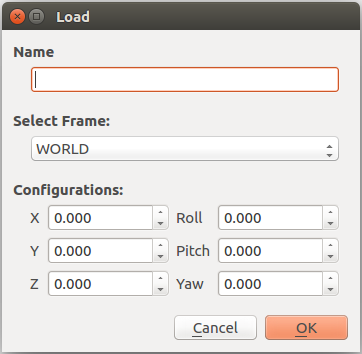
\includegraphics[scale=0.7]{Figures/EasyInsertLoadDialog.png}
         \caption{Device insertion dialog window}\label{fig:loadDialog}
       \end{subfigure}\\[\baselineskip]
       \begin{subfigure}[b]{\linewidth}
	    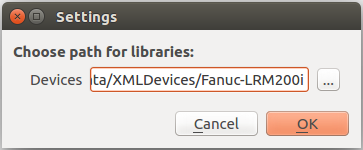
\includegraphics[scale=0.7]{Figures/settingsDialogWindow.png}
         \caption{Settings of device path dialog window}\label{fig:settingsDialog}
       \end{subfigure}
     \end{minipage}
     \caption{Three, out of many, dialog windows the user can experience and interact with when using EasyInsert.}\label{fig:EasyInsertDialogs}
\end{figure}

The Geometries tab shows a grid of icons, see figure~\ref{fig:EasyInsertGeo}. These icons represent either geometric primitives or frames that can be inserted into the WorkCell. Currently there are the following objects in the geometric tab, from top row to bottom:
\begin{enumerate*}[font={\color{red!50!black}\bfseries}]
\item Cube.
\item Cylinder.
\item Cone.
\item Plane.
\item Sphere.
\item Tube.
\item Fixed frame.
\item Movable frame.
\end{enumerate*}
These icons are all buttons the user can click, and after a click has occurred a dialog window appears with options regarding the insertion of said geometry. When the user hovers over a button, a small box identifying the icon appears, telling the user what sort of object it is. Figure~\ref{fig:cubeDialog} is the dialog window prompted when clicking the cube icon, and as seen, the user can specify a name for the geometry, select a reference frame and set the displacement and rotation configurations, just like when inserting a device. Though for a geometric primitive, like the cube, the user can also specify the dimensions of the geometric figure. The user can also specify whether the primitive should create a movable frame to associate the object with, or if the user want to use an existing frame.\\

The delete tab, as seen on figure~\ref{fig:EasyInsertDelete}, is a tab where the user can select a device, object or a frame and press the Delete button to remove said item from the WorkCell. The Devices list, shown in the delete tab, shows a device name. This means that when the user deletes a device, the frames associated with that device are now "free", i.e. the device property is deleted, but the frames and objects are still in the WorkCell. These object and frames will now show up in the Object list and the Frames list of the delete tab, and the user can now remove the frames and objects from the WorkCell. The Object list of the delete tab only deletes objects, but if the user selects a frame from the Frame list and deletes it, all objects associated with that frame will also be deleted. Furthermore, if the user selects a frame from the Frames list and deletes it, all children of children of said frame will also be deleted. It should be noted, that the Frames list of the delete tab does not update properly because of an internal bug in RWS, this means that when the user deletes a frame, the frame will still appear in the list, but if the user looks in the TreeView plugin, or searches the WorkCell, the user will notice that the frame has actually been deleted. The user is then able to delete a frame twice, which will cause a segmentation error and crash RWS. This is a critical error, but it has not been solved because solving this error is out of the scope of the project.



\subsection{Dialog Windows}
\label{sec:DialogWindows}
The dialog window is the main communication with the user in this plugin. Dialog windows are top-level windows, and they provide the user with either information, or they allow the users to select options to perform a command or task. This section will show how dialog windows has been handled in the plugin.\\

The dialogs of EasyInsert has been implemented in it's own class dialog.hpp, i.e. a subclass of QDialog, see figure~\ref{fig:subClassQWidget} for an example of a Qt subclass. This was done to keep it independent and self-contained from the rest of the plug-in. The constructor for the dialog class is very simple, see figure~\ref{fig:dialogConstructor}. A constructor with no WorkCell parameter is also available and passing a parent is optional, though a name must always be given to the constructor. 

\begin{figure}[h] % Code of dialog constructor
\centering
\lstset{language=C++} 
\begin{lstlisting}[frame=single]  
dialog::dialog(rw::models::WorkCell::Ptr wc, QString dialog, QWidget *parent)
    : QDialog(parent)
{
    _workCell = wc;
    mainLayout = new QVBoxLayout();
    setWindowTitle(dialog);
}			 
\end{lstlisting}
\caption{The dialog class constructor. A WorkCell pointer to a RW instance is passed along as a parameter. The QString parameter is the name of the dialog box and the QWidget is a pointer to the parent widget }
\label{fig:dialogConstructor} 	
\end{figure}

The dialog class is fairly simple to use and extend. A dialog is made of blocks in a vertical layout of QWidget's, i.e. a dialog instance is a composite widget containing composite widgets. Figure~\ref{fig:dialogWindowExample} shows a dialog window with four blocks initialised.

\begin{figure}[h]
	\centering
	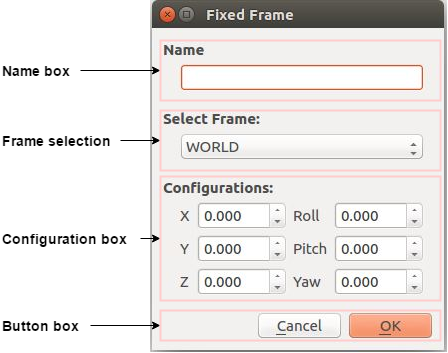
\includegraphics[scale=0.55]{Figures/dialogclassblocks.png}
	\caption{This figure shows a dialog window of adding a fixed frame to a WorkCell containing various widgets relevant to the action. }
	\label{fig:dialogWindowExample}
\end{figure}

All the blocks used to create all the dialog windows in the plug-in are shown in figure~\ref{fig:dialogBlocks}. These blocks are just member functions of the dialog class which returns a composite widget. So to create a dialog window as shown on figure~\ref{fig:dialogWindowExample}, a dialog instance should be constructed (in this case with a WorkCell pointer) and then simply adding the blocks to the dialog with the utility member function addToDialog(). See figure~\ref{fig:dialogWindowCode} which shows a code example on how to use the dialog class to construct the dialog window as shown on figure~\ref{fig:dialogWindowExample}. Since the dialog class is a subclass of QDialog, the position of the dialog window (opposed to a normal QDialog object) is always centred to the main application (RWS), even though a parent is passed as a parameter.

\begin{figure}[h] % code of adding stuff to a dialog
\centering
\lstset{language=C++} 
\begin{lstlisting}[frame=single]  
QString st = "Fixed Frame"; //Name of the dialog window
rw::models::WorkCell::Ptr wc = getRobWorkStudio()->getWorkCell(); //WorkCell
dialog* geoDialog = new dialog(wc,st,this); //Create the dialog window
geoDialog->addToDialog(geoDialog->createNameBox()); //Adding something
geoDialog->addToDialog(geoDialog->createFrameSelection());
geoDialog->addToDialog(geoDialog->createConfigurationBox());
geoDialog->addToDialog(geoDialog->createButtonBox());	
geoDialog->exec(); //execute/open dialog window	 
\end{lstlisting}
\caption{A sample code to illustrate how to construct the dialog window from figure~\ref{fig:dialogWindowExample}.}
\label{fig:dialogWindowCode} 	
\end{figure}

exec(), seen on figure~\ref{fig:dialogWindowCode} line 8, is an inherited public slot that executes/shows the dialog window. The dialog shown is in modal mode, meaning the window denies all user actions on any other widgets in the application. The function returns a DialogCode containing the information about whether the dialog window was accepted or rejected. The accepted or rejected information is determined by the user input to the createButtonBox() function block, since the OK button emits a accepted() signal to the accept() slot of the dialog object when pressed. Likewise the Cancel emits a rejected() signal to the reject() slot of the dialog object, though a rejected() signal is also emitted when the user presses ESC on the keyboard or the x(close) button of the dialog window. 

So when a dialog window has been created and used by a user, then some functionality should be executed based on the inputs given to the dialog. That means when the function exec() returns, we need to know whether the user accepted or rejected the dialog window (pressed OK or Cancel). This is done with the inherited public function result(). The function result() returns QDialog::Accepted when the dialog was accepted and QDialog::Rejected when it was rejected (QDialog::Accepted and QDialog::Rejected are both just normal enumerators, i.e. 1 and 0). 

\begin{figure}[h] % code of what to do after exec
\centering
\lstset{language=C++} 
\begin{lstlisting}[frame=single]  
geoDialog->exec();
if(geoDialog->result() == QDialog::Accepted) //Check the result
{
	std::string name = geoDialog->getNameBox(); //Get the name input
	std::string frame = geoDialog->getFrameSelection(); //Get frame selc
											 
		/*	Do something with the information    */ 
		
}
delete geoDialog; //Delete the dialog object when done using it
\end{lstlisting}
\caption{A sample code illustrating what to do after the exec()function returns.}
\label{fig:dialogAcceptedRejectedCode} 	
\end{figure}

As seen on figure~\ref{fig:dialogAcceptedRejectedCode}, after the exec() function returns, we simply check whether the result was QDialog::Accepted or not. If the result is accepted, then something should be done with the inputs given to the dialog window. We access these input via self explanatory public get-functions, e.g. the NameBox contains the name input (as seen on figure~\ref{fig:dialogAcceptedRejectedCode} line 4). After we have collected all the information we wanted out of the dialog window, then we can proceed to do something with the information, like e.g. the insertion of a frame. When we are done with the dialog window it should be deleted, because the dialog object is still alive until the parent is dead (in this case the plugin). If we do not delete the dialog object the dialog objects, created in the lifetime of the plugin, will just waste space in memory. 

It would to much time to inspect all of the function blocks on figure~\ref{fig:dialogBlocks}. Therefore only one function block, namely createNameBox() figure~\ref{fig:dialogCreateNameBoxCode} will be inspected. All the function blocks has a similar structure.

\begin{figure}[h] % code example of createNameBox
\centering
\lstset{language=C++} 
\begin{lstlisting}[frame=single]  
QWidget* dialog::createNameBox() {
    QGroupBox* nameBox = new QGroupBox(tr("Name")); //The nameBox widget
    QHBoxLayout *layout = new QHBoxLayout; //layout for the nameBox
    nameLine = new QLineEdit(); //The line edit the user can type the name
    layout->addWidget(nameLine); //Add the line edit to the layout
    nameBox->setLayout(layout); //Set the layout to the namebox
    return nameBox; //Return the nameBox
}
\end{lstlisting}
\caption{This figure shows the pulic function createNameBox() from the dialog class. The function is used to add a name line edit to dialog windows.}
\label{fig:dialogCreateNameBoxCode} 	
\end{figure}

The general procedure in the function blocks, as seen on figure~\ref{fig:dialogCreateNameBoxCode}, is to first create the composite widget. This widget, in the case of createNameBox, is a QGroupBox widget. QGroupBox is a widget that is mainly used as a composite widget. The QGroupBox provides a box to group widgets in, a frame if wanted and a title. As seen on figure~\ref{fig:dialogCreateNameBoxCode} line 2, the title is set upon construction with the string "Name". The tr() function is for translation purposes \cite{QtDocumentationTr}.
After the composite widget has been created, the layout for the parent widget has to be chosen and the child widget(s), in this case a QLineEdit(), has to be created. QLineEdit() is a simple line where text can be typed and edited in. When all the child widgets has been created, they need to be added to the layout of the parent. Lastly the layout is set to the parent and the parent is then returned. It should be noted that when the QLineEdit() was created, figure~\ref{fig:dialogCreateNameBoxCode} line 4, no parent was defined, i.e. it is actually not a child widget but a top-level widget. This is fine though, because when a top-level widget is added to a layout of another widget, that widget automatically takes responsibility as a parent and the top-level widget is now a child of that widget.

\begin{figure}[h] % table of function blocks
\centering
\begin{center}
  \begin{tabular}{ | p{6cm} | p{7cm} |}
    \hline
    \textbf{Function blocks} 	   &   \textbf{Description}  \\ \hline
    createButtonBox()			   &   The Cancel and OK buttons. This block is used in all the dialog windows.   		\\ \hline
    createNameBox() 			   &   A line edit to specify a name.   		\\ \hline
    createCheckFramesBox()		   &   Two exclusive check boxes, i.e. only one of the boxes can be checked at a time.		\\ \hline
    createConfigurationBox() 	   &   The different configurations available to adjust regarding displacement and rotation of the inserted element. 		\\ \hline
	createConfigurationBoxCube()   &   A cube specific configuration option, i.e. the dimensions of the cube.  	\\ \hline	    
	createConfigurationBoxSphere() &   A sphere specific configuration option, i.e. the dimensions of the sphere. 	\\ \hline	
	createConfigurationBoxCone()   &   A cone specific configuration option, i.e. the dimensions of the cone.  	\\ \hline	
    createConfigurationBoxTube()   &   A tube specific configuration option, i.e. the dimensions of the tube.  	\\ \hline	
	createLibSettingsBox(PropertyMap *map)		   &   This block is used to edit the settings of the device library.    	\\ \hline	 
	createFrameSelection()		   &   A way to select a parent frame for the inserted element. Default is the WORLD frame.		\\
    \hline
  \end{tabular}
\end{center}
\caption{This table summarizes all the different dialog function blocks used to construct the dialog windows in the plug-in.}
\label{fig:dialogBlocks} 
\end{figure}


Something about what could be worked on in regard to this class. Like constructors for a generic dialog window, mainlayout in a grid instead and extended adddialog functionality.
Is this something that should be in this chapter?


\subsection{EasyInsert Implementation}
This chapter will go through how EasyInsert achieved the functionalities and interfaces mentioned in section~\ref{sec:UserInterface} with the help from the dialog, creator and loader classes. 

Go through the constructor.

\begin{figure}[h] % Code of ei constructor
\centering
\lstset{language=C++} 
\begin{lstlisting}[frame=single]  
EasyInsert::EasyInsert():
    RobWorkStudioPlugin("EasyInsert", QIcon(":/pa_icon.png"))
{
    setupSettings();
    QScrollArea *widg = new QScrollArea(this);
	widg->setWidgetResizable(true);
	QWidget *dockWidgetContent = new QWidget(this);
	QVBoxLayout *verticalLayout = new QVBoxLayout(dockWidgetContent);
    _toolBar = createToolBar();
    verticalLayout->addWidget(_toolBar);
    verticalLayout->setAlignment(_toolBar,Qt::AlignRight);
    QTabWidget *tabWindow = new QTabWidget(dockWidgetContent);
    tabWindow->addTab(createDevTab(), "Devices");
    tabWindow->addTab(createGeoTab(), "Geometries");
    tabWindow->addTab(createDeleteTab(), "Delete");
    verticalLayout->addWidget(tabWindow);
    dockWidgetContent->setLayout(verticalLayout);
    widg->setWidget(dockWidgetContent);
	this->setWidget(widg);
}
\end{lstlisting}
\caption{The createDevTab() function. It creates the widget in the tab from figure~\ref{fig:EasyInsertDevice}}
\label{fig:eiConstructor} 	
\end{figure}

\subsubsection{Settings}
\label{sec:Settings}
Defining settings for an application is a common thing. It was therefore decided that EasyInsert should have some way to set settings. Settings for the plugin is stored in a XML file. The only current setting a user can set is, as mention in~\ref{sec:UserInterface}, the path for the library in the device tab. Though it should be easy to extend the plugin to have more settings, and even other utilities through the tool bar if needed.\\

The first thing the plugin does under it's construction, is to load the settings. This is done through the setupSettings() function, and the code of the function can be seen on figure~\ref{fig:settingsCodeSetup}. It is determined if there exists a settings file for the plugin (eisettings.xml), this is done on line 1 and 2 on figure~\ref{fig:settingsCodeSetup} with the boost library \cite{BoostPathSettings}. If a settings file exists, the code will proceed to load the file and warn the user if something went wrong. The loading of the file is done with the XMLPropertyLoader class \cite{XMLPropertyLoader}, which loads the settings file into a Property container called a PropertyMap. The PropertyMap class is part of the common namespace and can be used to store various user information, in this case for settings purposes. As seen on figure~\ref{fig:settingsCodeSetup} line 4, the PropertyMap, \_propMap, is loaded with the settings for the plugin. On line 13 we store a pointer, \_settingsMap, to the PropertyMap of the conveniently named Property EasyInsertSettings from the settings file. The following code checks if any settings were actually loaded, since if the user has not used the plugin yet, no settings files exists yet (or maybe it was deleted). The EasyInsertSettings Property would then have to be added, as seen on line 15, so a proper settings file can be created later. Settings are then stored under this property with an appropriate tag, so it is easy identifiable.

\begin{figure}[h] % Code of setupSettings
\centering
\lstset{language=C++} 
\begin{lstlisting}[frame=single]  
boost::filesystem::path settingsPath("eisettings.xml"); 
if( exists(settingsPath) ){ //If the file exists
	try { 
		_propMap = rw::loaders::XMLPropertyLoader::load("eisettings.xml");
		} catch(rw::common::Exception &e){
			RW_WARN("Could not load settings from 'eisettings.xml': " 
			<< e.getMessage().getText() << "\n Using default settings!");
		} catch(std::exception &e){
 			RW_WARN("Could not load settings from 'eisettings.xml': " 
 			<< e.what() << "\n Using default settings!");
		}
	}
_settingsMap = _propMap.getPtr<PropertyMap>("EasyInsertSettings");
if(_settingsMap==NULL){ // if there is no settings set yet
	_propMap.add("EasyInsertSettings", "Settings for EasyInsert", PropertyMap());
	_settingsMap = _propMap.getPtr<PropertyMap>("EasyInsertSettings");
}	 
\end{lstlisting}
\caption{Code example of how the settings of the plugin are loaded. If there were any trouble loading the settings, the user will be noticed and default settings will be used.}
\label{fig:settingsCodeSetup} 	
\end{figure}

As mentioned in section~\ref{sec:UserInterface}, the user is prompted with a dialog window when pushing the [...] button on figure~\ref{fig:settingsDialog}. This is a QFileDialog \cite{QtDocumentationQFileDialog} dialog which allow users to select a directory. The createLibSettingsBox(PropertyMap *map) function from figure~\ref{fig:dialogBlocks}, the function block that is part of figure~\ref{fig:settingsDialog} , signals the public slot setDirectoryDialog() on a click event of the [...] button. On figure~\ref{fig:settingsCodeQFileDialog} the code from the setDirectorydialog() slot is shown. The QFileDialog instance saves the directory the user choose in the QString dir on line 1, and we then make sure on line 4 that the user didn't select nothing(if he cancels the dialog). The directory is then set in the \_settingsMap on line 5 using the PropertyMap member function set(const std::string \&identifier, const T \&value ). The identifier is here "Devices" and the value associated with it is the chosen directory dir. Finally the pathLine, the line edit of figure~\ref{fig:settingsDialog}, is updated as well.

\begin{figure}[h] % Code of QFileDialog and setting the setting
\centering
\lstset{language=C++} 
\begin{lstlisting}[frame=single]  
QString dir = QFileDialog::getExistingDirectory(this, 
		tr("Open Directory"), pathLine->text(),
	    QFileDialog::ShowDirsOnly | QFileDialog::DontResolveSymlinks);
    if (dir != "") {
        _settingsMap->set("Devices", dir.toStdString());
        pathLine->setText(dir);
    }
\end{lstlisting}
\caption{The setDirectoryDialog() function. This function prompts the user with a QFileDialog dialog window, which allow users to select directory. The selected directory is then set in the settings and the pathLine of the LibSettingsBox is updated.}
\label{fig:settingsCodeQFileDialog} 	
\end{figure}

When the settings dialog from figure~\ref{fig:settingsDialog} returns, it is checked if the user accepted the settings,  as seen on figure ~\ref{fig:settingsCodeReturnDialog}. If the user accepted we try to save the settings using the XMLPropertySaver \cite{XMLPropertySaver} class and catch any errors. The root path is then updated (see section~\ref{sec:DeviceTab} for more information about the root path) with the PropertyMap member function get(const std::string \&identifier, const T \&defval). "Devices" is here the identifier, that means, if a Device tag exists in the \_settingsMap, then the associated setting is returned. Otherwise the default value "/" is returned.

\begin{figure}[h] % Code of save the settings, and getting
\centering
\lstset{language=C++} 
\begin{lstlisting}[frame=single]  
if (settingsDialog->result() == QDialog::Accepted) {
	try {
		rw::loaders::XMLPropertySaver::save(_propMap, "eisettings.xml");
	} catch(const rw::common::Exception& e) {
		RW_WARN("Error saving settings file: " << e);
	} catch(...) {
		RW_WARN("Error saving settings file due to unknown exception!");
	}
	view->setRootIndex(dirmodel->setRootPath(QString::fromStdString(_settingsMap->get("Devices", "/")))); 
}
\end{lstlisting}
\caption{Example code of when a settings dialog window has returned and something should be done to the settings.}
\label{fig:settingsCodeReturnDialog} 	
\end{figure}

Reflection, we should have added to the rwsettings file, the reason we did not was, because that at that moment, it was actually more easy to make our own settings file.

\subsubsection{Tool Bar}
\label{sec:ToolBar}
The settings button, as noted in~\ref{sec:UserInterface}, is the only button available in the tool bar so far, and thus the extend of the tool bar will be shortly discussed in this chapter.
The tool bar is constructed in the createToolBar() function (figure~\ref{fig:settingsToolBarCode}) and it is pretty straight forward. The only hiccup can be managing the menu's for the buttons in the tool bar. We create a tool bar with the QToolBar class and the buttons with QToolButton. After the toolbar and button(s) has been created, the icons and tool tips are set. On line 5 a QMenu is created, QMenu is a selection menu. Afterwards a QAction is created as well, which is an abstract user interface action that can be inserted into widgets. We then add the action to the menu. On line 8 the settingsButton gets the menu set, followed by a pop up mode selection. Lastly we add the settingsButton to the toolBar, and we connect the settingsAction to the settings() slot. The settings() slot is the function that creates the settings dialog window on figure~\ref{fig:settingsDialog} and waits for the user to select the settings, before saving them, like on figure~\ref{fig:settingsCodeReturnDialog}.

\begin{figure}[h] % Code of createToolBar
\centering
\lstset{language=C++} 
\begin{lstlisting}[frame=single]  
QToolBar *toolBar = new QToolBar(this);
QToolButton *settingsButton = new QToolButton();
settingsButton->setIcon(QIcon(":/settings.png"));
settingsButton->setToolTip("Settings");
QMenu *settingsMenu = new QMenu("Settings menu");
QAction *settingsAction = new QAction("Libraries",this);
settingsMenu->addAction(settingsAction);
settingsButton->setMenu(settingsMenu);
settingsButton->setPopupMode(QToolButton::InstantPopup);
toolBar->addWidget(settingsButton);
connect(settingsAction, SIGNAL(triggered()), this, SLOT(settings()));
return toolBar;
\end{lstlisting}
\caption{The createToolBar() function. This function sets up the tool bar in the plugin and connects the actions to the appropriate slots.}
\label{fig:settingsToolBarCode} 	
\end{figure}

Reflection
the undo button would have been another button on the tool bar

\subsubsection{Devices Tab}
\label{sec:DeviceTab}
This section discusses the implementation of the Devices tab from figure~\ref{fig:EasyInsertDevice}. The Devices tab is set up with the function createDevTab(), which returns the composite widget making up the Devices tab. createDevTab() can be seen on figure ~\ref{fig:deviceTabCode}. The widget created and returned is a QScrollArea widget with a composite child. A QScrollArea widget provides a scrolling view onto another widget (the child). The QScrollArea widget is created on line 2, the widget is then set to be resizeable and the frame is removed. When a QScrollArea is set to be resizeable, the child widget of the QScrollArea will automatically be resized so to either avoid scroll bars (decrease size of child) or utilize extra space (increase size of child). It should be noted that when QScrollArea has a composite child with a layout, the size policy of that layout will determine the size (or resize) of the widget. The composite child is created on line 5 and then a vertical layout is created. On line 7 a QListView is created, this is a widget that provides a list view onto a model. Afterwards a QFileSystemModel is created and put onto the list view. The QFileSystemModel provides a data model for the local file system. Following, the \_settingsMap with the Devices library path is read, and then used to set the root path on the model with the QFileSystemModel public function setRootPath(const QString \&newpath). This actually installs a QFileSystemWatcher to monitor the path and update the QFileSystemModel accordingly. The view of the QListView's root index is then set to the model's root path. The load button is then created and connected to the loadDevice() slot which creates the dialog window shown on figure~\ref{fig:loadDialog}. Finally the widgets, the view and the button, are added to the layout and the composite widget gets the layout set. The composite widget has now been made, so the QScrollArea is then imposed onto the composite widget and returned. 

\begin{figure}[h] % Code of createDevTab()
\centering
\lstset{language=C++} 
\begin{lstlisting}[frame=single]  
QWidget* EasyInsert::createDevTab(){
	QScrollArea *widg = new QScrollArea(); //the parent 
	widg->setWidgetResizable(true); //children will scale 
	widg->setFrameShape(QFrame::NoFrame); //no frame 
	QWidget *devTab = new QWidget(); //container widget
	QVBoxLayout *verticalLayout = new QVBoxLayout(devTab); 
	view = new QListView(devTab); //list view widget
	dirmodel = new QFileSystemModel(view); //filesystem model
	view->setModel(dirmodel); //set the model
	view->setRootIndex(dirmodel->setRootPath(QString::fromStdString(_settingsMap->get("Devices", "/")))); // set the root
	QPushButton *loadBtn = new QPushButton("Load",devTab); //make button
	connect(loadBtn, SIGNAL(clicked()), this, SLOT(loadDevice())); 
	verticalLayout->addWidget(view); // add to layout
	verticalLayout->addWidget(loadBtn);
	devTab->setLayout(verticalLayout); //set the layout
	widg->setWidget(devTab); // set the widget
	return widg;
}
\end{lstlisting}
\caption{The createDevTab() function. It creates the widget in the tab from figure~\ref{fig:EasyInsertDevice}}
\label{fig:deviceTabCode} 	
\end{figure}

\subsubsection{Geometries Tab}
\label{sec:GeoTab}

Introduction

The Geometries tab is set up with the function createGeoTab() (figure ~\ref{fig:geoTabCode}), and it uses a similar procedure as the createDevTab(). A QScrollArea with a composite widget is returned. The main difference between the Devices tab and the Geometries tab, are the children of the composite widget, a QGridLayout, and that the QScrollArea is not set to be resizeable. The reason for different children of the composite widget is quite obvious (this tab should show something else), and a QGridLayout was chosen because it is a convenient layout to present the buttons in. The resizeable option of the QScrollArea is not used because of aesthetic reasons. Since, if the resizeable option was on, the buttons could either be scaled to ridiculous sizes or, if the buttons have fixed sizes, have loads of spacing. 

The children of the composite widget are eight QToolButtons. Each button has an intuitive icon and size set, and a tool tip to reflect the action. The buttons are then connected to their appropriate slot function.    

slots are boilerplate code, they all create a prober dialog window so the user can select options for the action, the slot then waits for the dialog to return and then uses the creator with the user supplied parameters as discussed in the other sections.

QToolButton are more sophisticated and are generally preferred when the button is used as an icon.


\begin{figure}[h] % Code of createGeoTab()
\centering
\lstset{language=C++} 
\begin{lstlisting}[frame=single]  
QWidget* EasyInsert::createGeoTab(){
	QScrollArea *widg = new QScrollArea(); //the parent
    widg->setFrameShape(QFrame::NoFrame); //no frame
    QWidget *geoTab = new QWidget(); //container widget
    QGridLayout *layout = new QGridLayout(geoTab);
    QToolButton *btns[8]; //8 buttons

    btns[0] = new QToolButton();
    btns[0]->setIcon(QIcon(":icons/cube.png")); //btn icon
    btns[0]->setToolTip("Cube"); //tool tip
    btns[0]->setIconSize(QSize(50, 50)); // size of the btn
    	/*  Create all the other buttons the same way   */
    connect(btns[0], SIGNAL(clicked()), this, SLOT(cube()));
 		/*  Connect all the buttons to their slots as well  */
    layout->addWidget(btns[0], 0, 0);
		/*  Add all the other buttons to the grid as well  */    
  
    geoTab->setLayout(layout); //set layout
    widg->setWidget(geoTab); // set widget
    return widg;
}
\end{lstlisting}
\caption{The createGeoTab() function. It creates the widget in the tab from firgure~\ref{fig:EasyInsertGeo}. It should be noted that some redundant code has been omitted from the figure to save space.}
\label{fig:geoTabCode} 	
\end{figure}

\subsubsection{Delete Tab}
\label{sec:DelTab}


\begin{figure}[h] % Code of createDelTab()
\centering
\lstset{language=C++} 
\begin{lstlisting}[frame=single]  
QWidget* EasyInsert::createDelTab(){
	QScrollArea *widg = new QScrollArea(); //the parent
    widg->setWidgetResizable(true); //scale widgets
    widg->setFrameShape(QFrame::NoFrame); //no frame
    QWidget *devTab = new QWidget(); //container widget
    QVBoxLayout *verticalLayout = new QVBoxLayout(devTab);
    QGroupBox *delDevBox = new QGroupBox(tr("Devices:"));
    QGroupBox *delFrameBox = new QGroupBox(tr("Frames:"));
    QGroupBox *delObjBox = new QGroupBox(tr("Objects:"));
    QGridLayout *layoutDev = new QGridLayout();
    QGridLayout *layoutFrame = new QGridLayout();
    QGridLayout *layoutObj = new QGridLayout();
    _deviceWidget = new QListWidget(this); //list widgets 
    _frameWidget = new QListWidget(this);  //to list relevant
    _objectWidget = new QListWidget(this); //items

    QPushButton *delDevBtn = new QPushButton("Delete",devTab);
    connect(delDevBtn, SIGNAL(clicked()), this, SLOT(deleteDev()));
    /* create the two other delete buttons and connect them as well */

    layoutDev->addWidget(_deviceWidget,0,0); //left side
    layoutDev->addWidget(delDevBtn,0,1); // right side
    delDevBox->setLayout(layoutDev);
    /* add widget and set layout for the two others as well */

    verticalLayout->addWidget(delDevBox); //add all widgets
    verticalLayout->addWidget(delObjBox);
    verticalLayout->addWidget(delFrameBox);
    devTab->setLayout(verticalLayout); //set layout
    widg->setWidget(devTab); // set widget
    return widg;
}
\end{lstlisting}
\caption{The createDelTab function. It creates the widget in the tab from figure~\ref{fig:EasyInsertDelete}. It should be noted that some redundant code has been omitted from the figure to save space.}
\label{fig:delTabCode} 	
\end{figure}


QlistWidget


\subsubsection{The Slots}

Many slots. They all have been constructed fairly similar, except the delete ones.



